\section{Evaluación económica}\label{sec:economia}

\subsection{Costo del sistema}

El costo incluye los equipos, la estructura, los conductores, las protecciones, el diseño y la instalación (Tabla~\ref{tab:costos}). Las baterías se valoraron con el precio de Costa Rica \cite{kuat}; para los demás equipos no se encontraron precios publicados en el país, por lo que se usaron precios de lista de tiendas de Estados Unidos y Europa de octubre y noviembre de 2026 \cite{precio_modulo, precio_mppt, precio_mp, pes, elliott, standard, zoro}. Los dólares y euros se convirtieron con el tipo de cambio de referencia de venta del BCCR del 19 de noviembre de 2026, ¢447.54 por dólar, y 1.0997 dólares por euro \cite{bccr}. Las canalizaciones, los conductores de puesta a tierra y los accesorios se estimaron como un 15\,\% de los conductores y protecciones. Para el diseño se usaron los honorarios mínimos del arancel del CFIA, 4.5\,\% del valor de la obra \cite{cfia_arancel}, y para el registro del proyecto, 0.25\,\% \cite{cfia_registro}. Para la instalación no se encontraron valores públicos en Costa Rica, así que se supusieron ¢300\,000 de mano de obra y un 20\,\% de ganancia del instalador sobre el costo total.

\begin{table}[!htb]
\caption{Costo estimado del sistema}
\label{tab:costos}
\centering
\footnotesize
\setlength{\tabcolsep}{4pt}
\begin{tabular}{l r}
\toprule
Rubro & Monto [¢] \\
\midrule
Baterías Power Queen 24 V 200 Ah (4 $\times$ ¢850\,000) & 3\,400\,000 \\
Inversor-cargador MultiPlus-II (997.05 USD) & 446\,220 \\
Módulos AIKO 450 W (4 $\times$ 128.96 EUR) & 253\,876 \\
Regulador SmartSolar 150/85 (476.00 USD) & 213\,029 \\
Estructura de montaje (Tabla~\ref{tab:montaje}) & 134\,978 \\
Conductores & 279\,318 \\
Protecciones y tableros (Tabla~\ref{tab:protecciones}) & 505\,998 \\
Otros materiales eléctricos (15\,\%) & 117\,797 \\
\midrule
Subtotal de equipos y materiales & 5\,351\,216 \\
\midrule
Diseño, honorarios CFIA (4.5\,\%) & 254\,305 \\
Registro ante el CFIA (0.25\,\%) & 14\,128 \\
Instalación (supuesto) & 300\,000 \\
\midrule
Costo total & 5\,919\,648 \\
Ganancia del instalador (20\,\%) & 1\,183\,930 \\
\midrule
\textbf{Precio del sistema} & \textbf{7\,103\,578} \\
\bottomrule
\end{tabular}
\\[2pt]
{\footnotesize Equivale a 15\,872 USD. No incluye flete, nacionalización ni IVA de los equipos importados. Las partidas están redondeadas al colón.}
\end{table}

Las baterías son el 48\,\% del precio. El costo real puede ser mayor, porque no se incluyeron el flete ni los impuestos de importación de los equipos, y debe confirmarse con cotizaciones de distribuidores locales.

\subsection{Ahorro en la factura}

Con el sistema, las cargas críticas dejan de tomar energía de la red, porque la energía disponible cubre su demanda todos los meses (Tabla~\ref{tab:energia}). La factura con el sistema se calculó con la misma tarifa (Tabla~\ref{tab:tarifa}), restando al consumo de cada mes la energía de las cargas críticas (Tabla~\ref{tab:facturas}). La factura anual baja de ¢236\,730 a ¢108\,565, un ahorro de ¢128\,165 (54\,\%). El ahorro es mayor que la proporción de energía, de 49\,\%, porque al bajar el consumo de unos \SI{270}{kWh} a unos \SI{140}{kWh} por mes desaparecen el bloque de ¢76.02/kWh y el IVA de los meses que superaban \SI{280}{kWh}. Este ahorro supone que el sistema funciona todos los días, no solo durante los cortes; si se usara solo como respaldo, el ahorro se limitaría a la energía consumida durante los cortes.

\subsection{Proyección financiera}

El flujo de caja se proyectó a 25 años con una tasa de descuento de 7\,\% y tarifas constantes. La degradación de los módulos, de 1\,\% el primer año y 0.35\,\% por año después \cite{aiko_ds}, no reduce el ahorro: en el año 25 la energía disponible baja 9.4\,\% y la cobertura de noviembre queda en 105\,\%, de modo que las cargas críticas se siguen cubriendo. Se supuso un mantenimiento de 1\,\% del precio por año (¢71\,036) y el reemplazo del inversor y el regulador en el año 13 (¢659\,249), porque sus fichas no declaran la vida útil. Las baterías se reemplazan en el año 15 (¢3\,400\,000): con una descarga diaria de 22\,\%, los 15\,000 ciclos que declara el fabricante al 60\,\% de DOD \cite{pq} no limitan su vida, pero el fabricante no declara la vida calendario.

\begin{figure}[!htb]
\centering
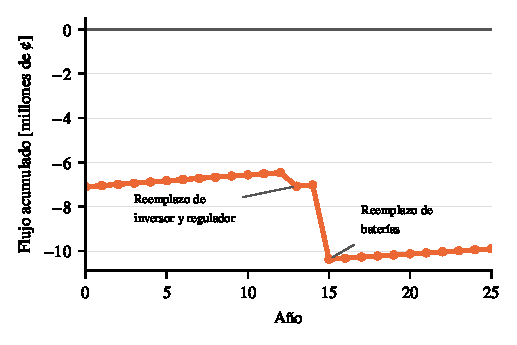
\includegraphics[width=\anchofig]{flujo_acumulado.pdf}
\caption{Flujo de caja acumulado del sistema.}
\label{fig:flujo}
\end{figure}

La Fig.~\ref{fig:flujo} muestra el flujo acumulado. El ahorro anual, ¢128\,165, supera el mantenimiento en ¢57\,129, de modo que el flujo acumulado sube unos ¢57\,000 por año, y los reemplazos lo bajan a ¢10.31 millones negativos en el año 15. Al final de los 25 años el flujo acumulado es de ¢9.73 millones negativos y el valor actual neto, de ¢7.94 millones negativos: la inversión no se recupera. Sin mantenimiento ni reemplazos, el tiempo de recuperación simple sería de $7\,103\,578/128\,165=55$ años.

El costo de la energía que entrega el sistema a las cargas críticas, calculado como el valor presente de los costos entre el valor presente de la energía, es de ¢512/kWh, frente al costo de la energía de la red en el bloque de más de \SI{200}{kWh}, de ¢76.02/kWh más alumbrado, bomberos e IVA. El resultado indica que el sistema no se justifica por el ahorro en la factura: su valor está en mantener funcionando la refrigeración, la iluminación y las comunicaciones durante dos días sin servicio eléctrico.
